\chapter{Survey layout and Questions}


These were the questions and answer options as used in Nettskjema survey. This was accessed via a specially created website, which had full details about the research and the ability to contact the researcher. 
https://aamccormack12.wixsite.com/sealevelextremes 

The survey was designed for access via smartphones, computers and tablets. The UI was checked on each of these machines and the first targeted recipients course mates and then test engineers, so that any issues could quickly be discovered and fixed. 

\section{Example Survey - English - Grillstad}

Do you consent to these answers being used for an MSc research project?
\begin{itemize}
	\item Yes
    \item No
\end{itemize}

\newpage

\paragraph{}
How long have you known this area?
\begin{itemize}
	\item > 30 years.
    \item > 20 years
    \item > 10 years
    \item > 5 years
    \item > 1 year
    \item < 1 year
\end{itemize}

\paragraph{}
What communities in this area are you part of?
\begin{itemize}
    \item marine worker
    \item non-marine worker
    \item resident
    \item student
    \item leisure user - land
    \item leisure user - water
    \item commuter
    \item other 
\end{itemize}
Other (Write in here)
\paragraph{}

This research investigates knowledge about extreme sea levels in Trondheim, focusing on storm surges. A storm surge occurs when the weather temporarily causes water to be forced up and onto the coast.

A 20-year storm surge refers to the probability of an event, meaning there is a 1 in 20 chance (5 percent) of this level of event every year. This expectation changes over time, for example due to climate change.
\newpage

What is your level of interest in sea level extremes?
\begin{itemize}
    \item professional interest
    \item high
    \item medium
    \item low
    \item low
    \item not interested
\end{itemize}
\paragraph{}

The following questions display simulated water levels extremes in Trondheim. The numbers in these images refer to the height above NN2000 which can be considered an approximation of mean sea level.
\paragraph{}
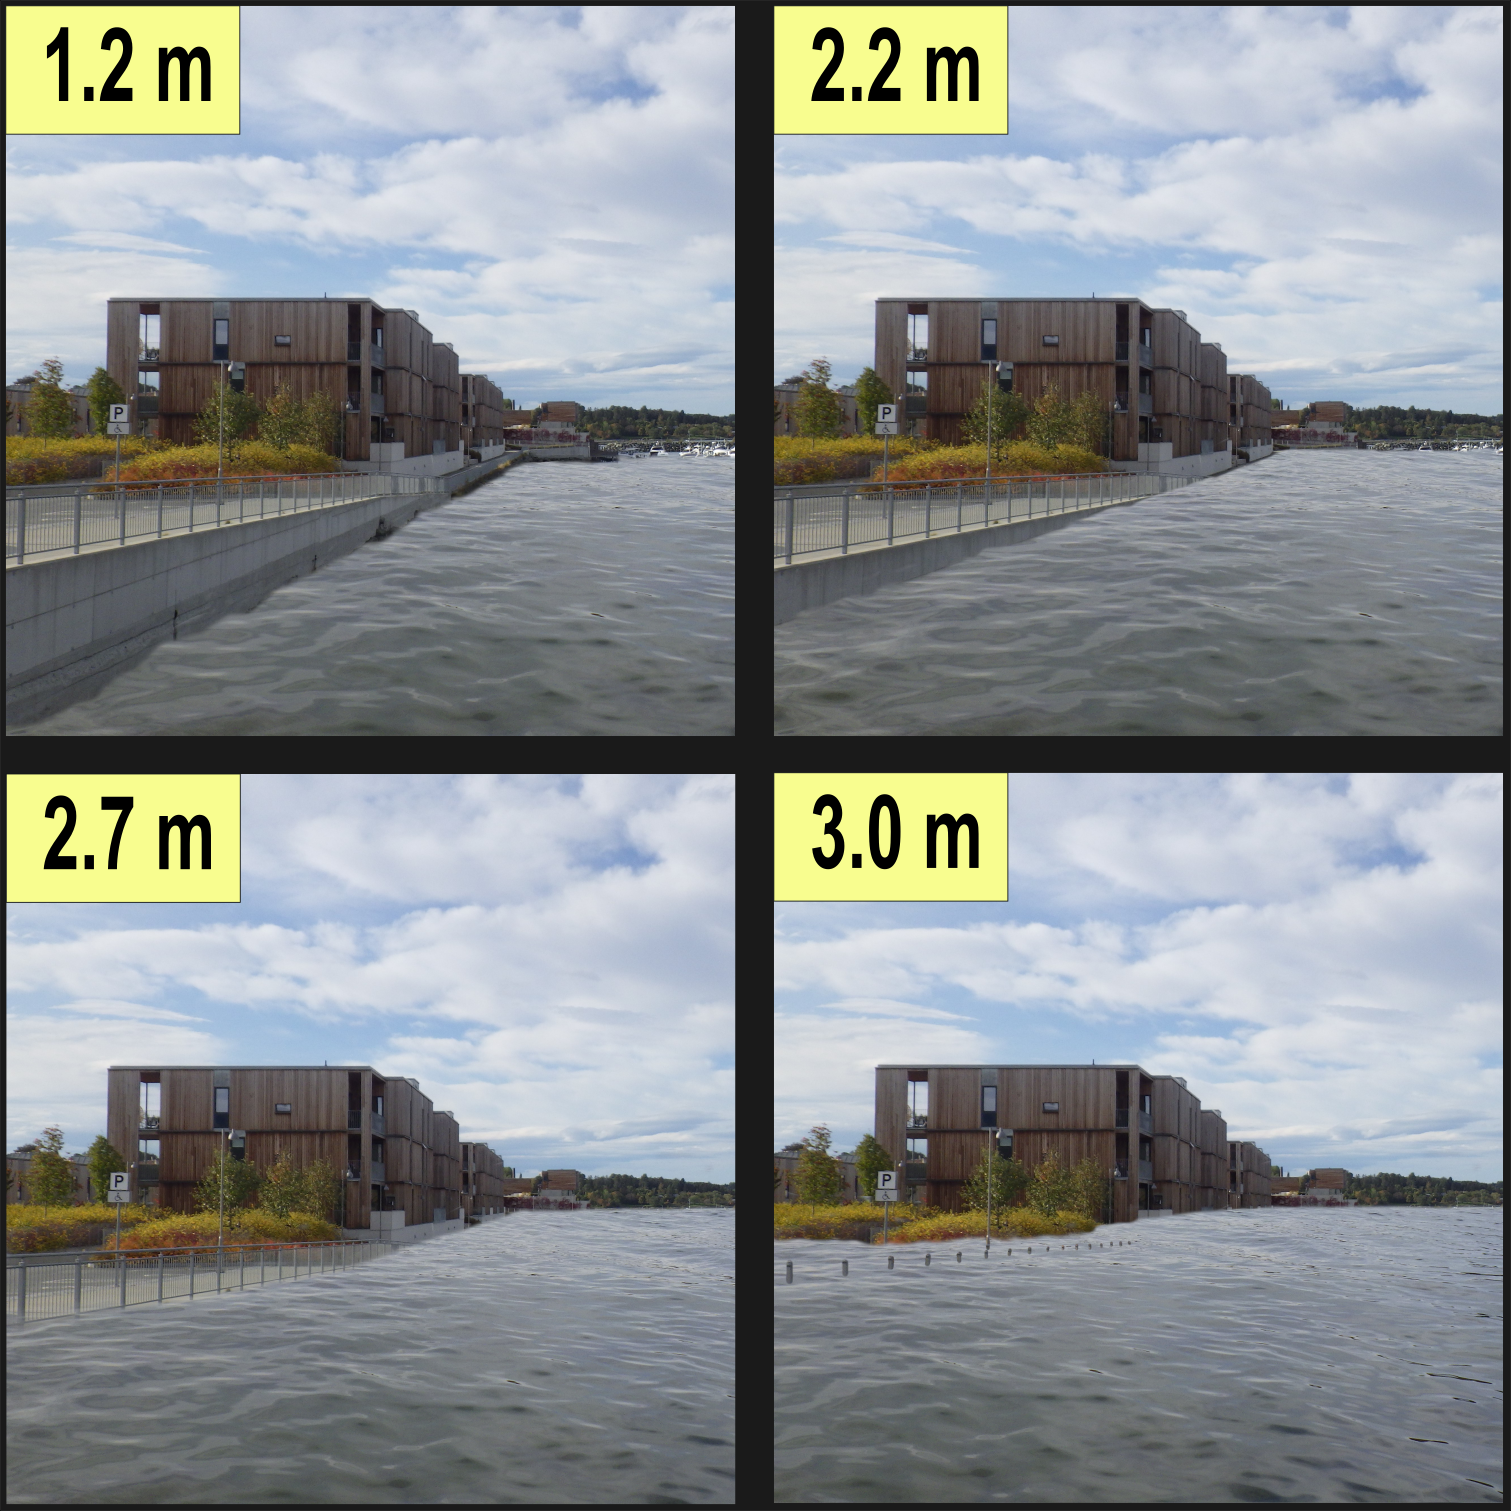
\includegraphics[width=1\textwidth]{fig_appendix/grillstad 2090 q.png}

Which image shows the current 20-year storm surge?
\begin{itemize}
    \item 1.2 m
    \item 2.2 m
    \item 2.7 m
    \item 3.0 m
\end{itemize}
\paragraph{}

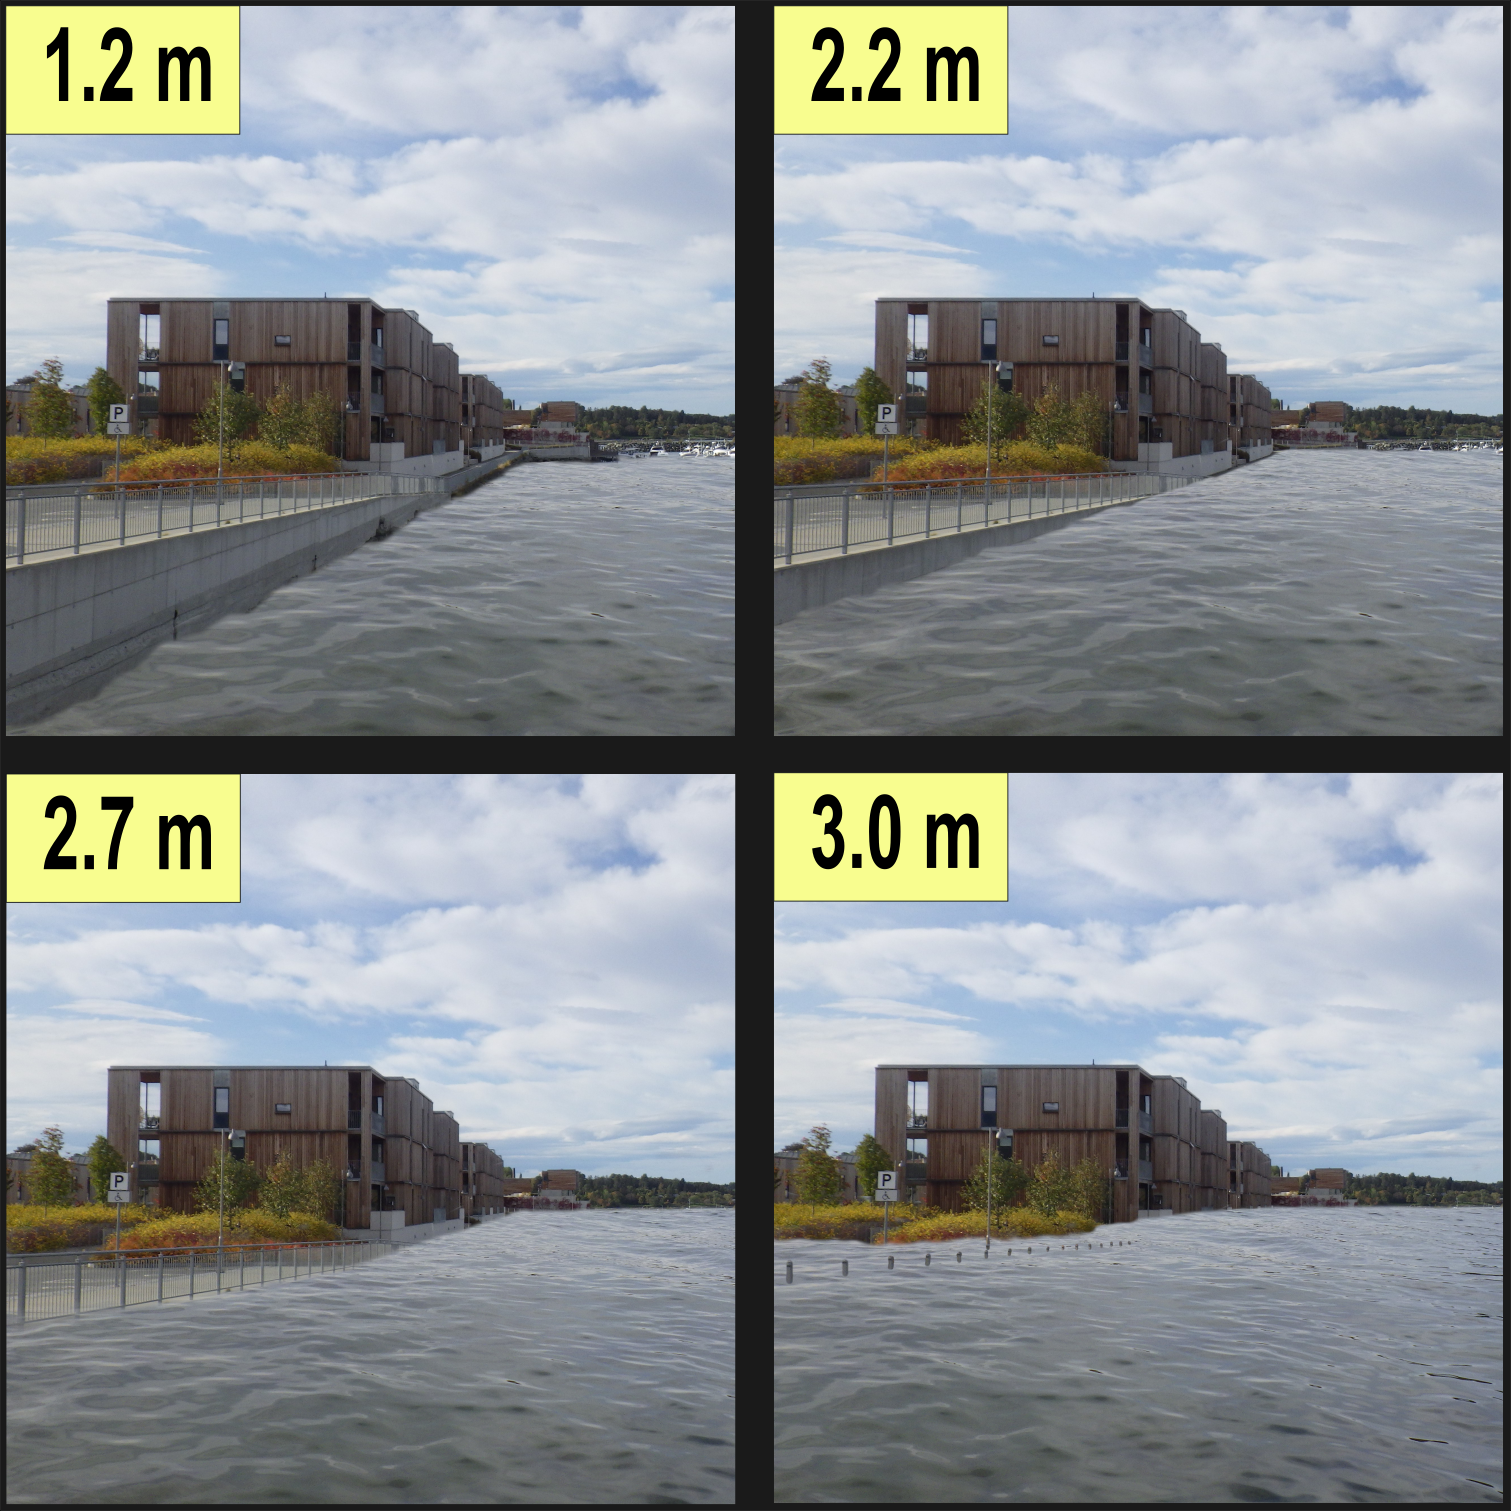
\includegraphics[width=1\textwidth]{fig_appendix/grillstad 2090 q.png}
Which image shows the 20-year storm surge projected for 2090?
\begin{itemize}
    \item 1.2 m
    \item 2.2 m
    \item 2.7 m
    \item 3.0 m
\end{itemize}
\paragraph{}

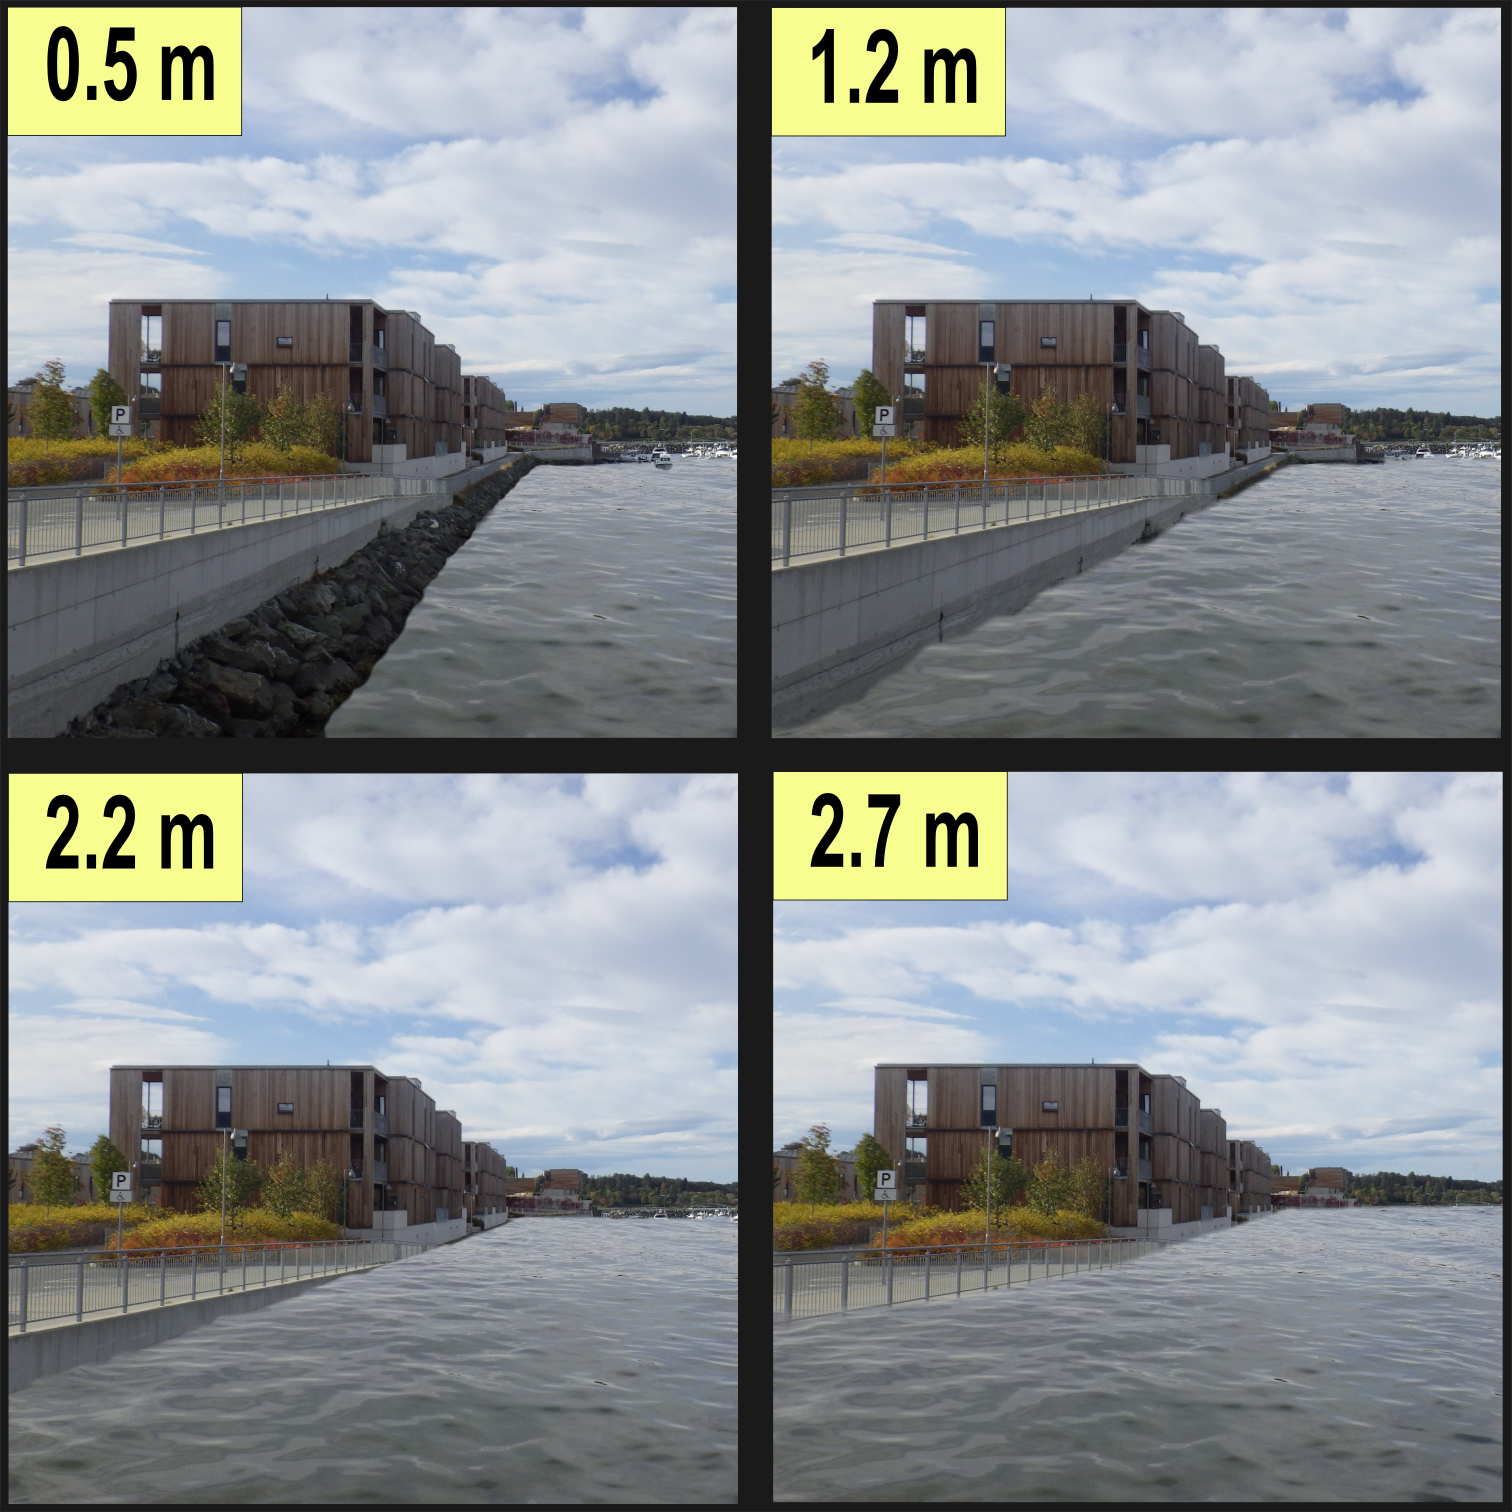
\includegraphics[width=1\textwidth]{fig_appendix/grillstad 2022 q.png}
Which image displays the current high tide?
\begin{itemize}
    \item 0.5 m
    \item 1.2 m
    \item 2.2 m
    \item 2.7 m
   \end{itemize}
\paragraph{}

Where do you get information about changes to this place?
e.g. subsidence, incidents, roadworks
\begin{itemize}
    \item personal observation
    \item family
    \item friends
    \item newspapers
    \item tv
    \item social media
    \item organisation membership
    \item municipality
\end{itemize}
\paragraph{}

Where do you get information about climate change?
\begin{itemize}
    \item personal observation
    \item family
    \item friends
    \item newspapers
    \item tv
    \item social media
    \item organisation membership
    \item peer-reviewed articles
    \item formal education
\end{itemize}

\paragraph{}
Are you concerned about climate change?
1 - not at all, 5 - very concerned
Rating Scale

\paragraph{}
How would flooding associated with sea level extremes in this area affect you?
\begin{itemize}
    \item no impact
    \item mild impact
    \item medium impact
    \item significant impact
\end{itemize}
If you would like to give more details on this, please write below.
\paragraph{}

How much do you think the sea level has changed here in the past 30 years?
\begin{itemize}
    \item + 50 cm
    \item + 20 cm
    \item + 10 cm
    \item no change
    \item - 10 cm
    \item - 20 cm 
    \item - 50 cm 
\end{itemize}
\paragraph{}

How much do you think the sea level will change in the next 30 years?
\begin{itemize}
    \item + 50 cm
    \item + 20 cm
    \item + 10 cm
    \item no change
    \item - 10 cm
    \item - 20 cm 
    \item - 50 cm 
\end{itemize}
\paragraph{}

Please tick if you remember any of these dates when coastal sea levels in Trondheim were over 2m.
\begin{itemize}
    \item 2020 February
    \item 2011 November
    \item 1999 November
    \item 1998 February
    \item 1997 February
    \item 1993 January
    \item 1990 February
    \item 1971 November
    \item I do not remember any of these events
\end{itemize}
\paragraph{}

From the following what are the major risks to people in this area?
\begin{itemize}
    \item shoreline instability
    \item storm surges
    \item waves
    \item strong winds
    \item strong tides
    \item drowning
    \item cold water shock
    \item I don't know
    \item I perceive no major risks
    \item human error
\end{itemize}
\paragraph{}

From the following what are the major risks to infrastructure in this area?
\begin{itemize}
    \item shoreline instability
    \item storm surges
    \item waves
    \item strong winds
    \item strong tides
    \item I don't know
    \item I perceive no major risks
    \item weathering
    \item precipitation
    \item human error
\end{itemize}

\paragraph{}
If you would like to give other examples of risk in this area, please write here.
\paragraph{}

How did you access this survey?
\begin{itemize}
    \item poster
    \item email
    \item social media
    \item via organisation membership
    \item via place of employment
    \item personal connection to researcher
\end{itemize}
\paragraph{}

If you would like further information on this research, please provide your e-mail address.
\newpage

\section{Example Survey - Norwegian - Brattøra }
Samtykker du at disse svarene brukes til masterforskning?
\begin{itemize}
    \item ja
    \item nei
\end{itemize}
\paragraph{}

Hvor lenge har du kjent dette området?
\begin{itemize}
	\item > 30 years.
    \item > 20 years
    \item > 10 years
    \item > 5 years
    \item > 1 year
    \item < 1 year
\end{itemize}
\paragraph{}

Hvilke samfunn i dette området er du en del av?
\begin{itemize}
    \item marinearbeider
    \item ikke-marin arbeider
    \item beboer
    \item student
    \item fritidsbruket - land
    \item fritidsbruket - vann
    \item pendler
    \item andre
\end{itemize}   

\paragraph{}
Denne forskningen undersøker kunnskap om ekstreme havnivåer i Trondheim, med fokus på stormflo. En stormflo oppstår når været midlertidig fører til at vann presses opp og inn på kysten. 
En 20-årig stormflo refererer til sannsynligheten for en hendelse. Det betyr at det er en sjanse på 1 av 20 (5 prosent) for dette nivået av begivenhet hvert år. Denne forventningen endres over tid, for eksempel på grunn av klimaendringer.
\paragraph{}

Hvor stor interesse har du for ekstreme havnivåer?
\begin{itemize}
    \item faglig interesse
    \item høy
    \item middels
    \item lav
    \item ikke interessert
\end{itemize}
\paragraph{}

Følgende spørsmål viser simulerte havnivå ekstremes i Trondheim. Tallene på disse bildene viser til høyden over NN2000 som kan betraktes som en tilnærming av gjennomsnittlig havnivå.

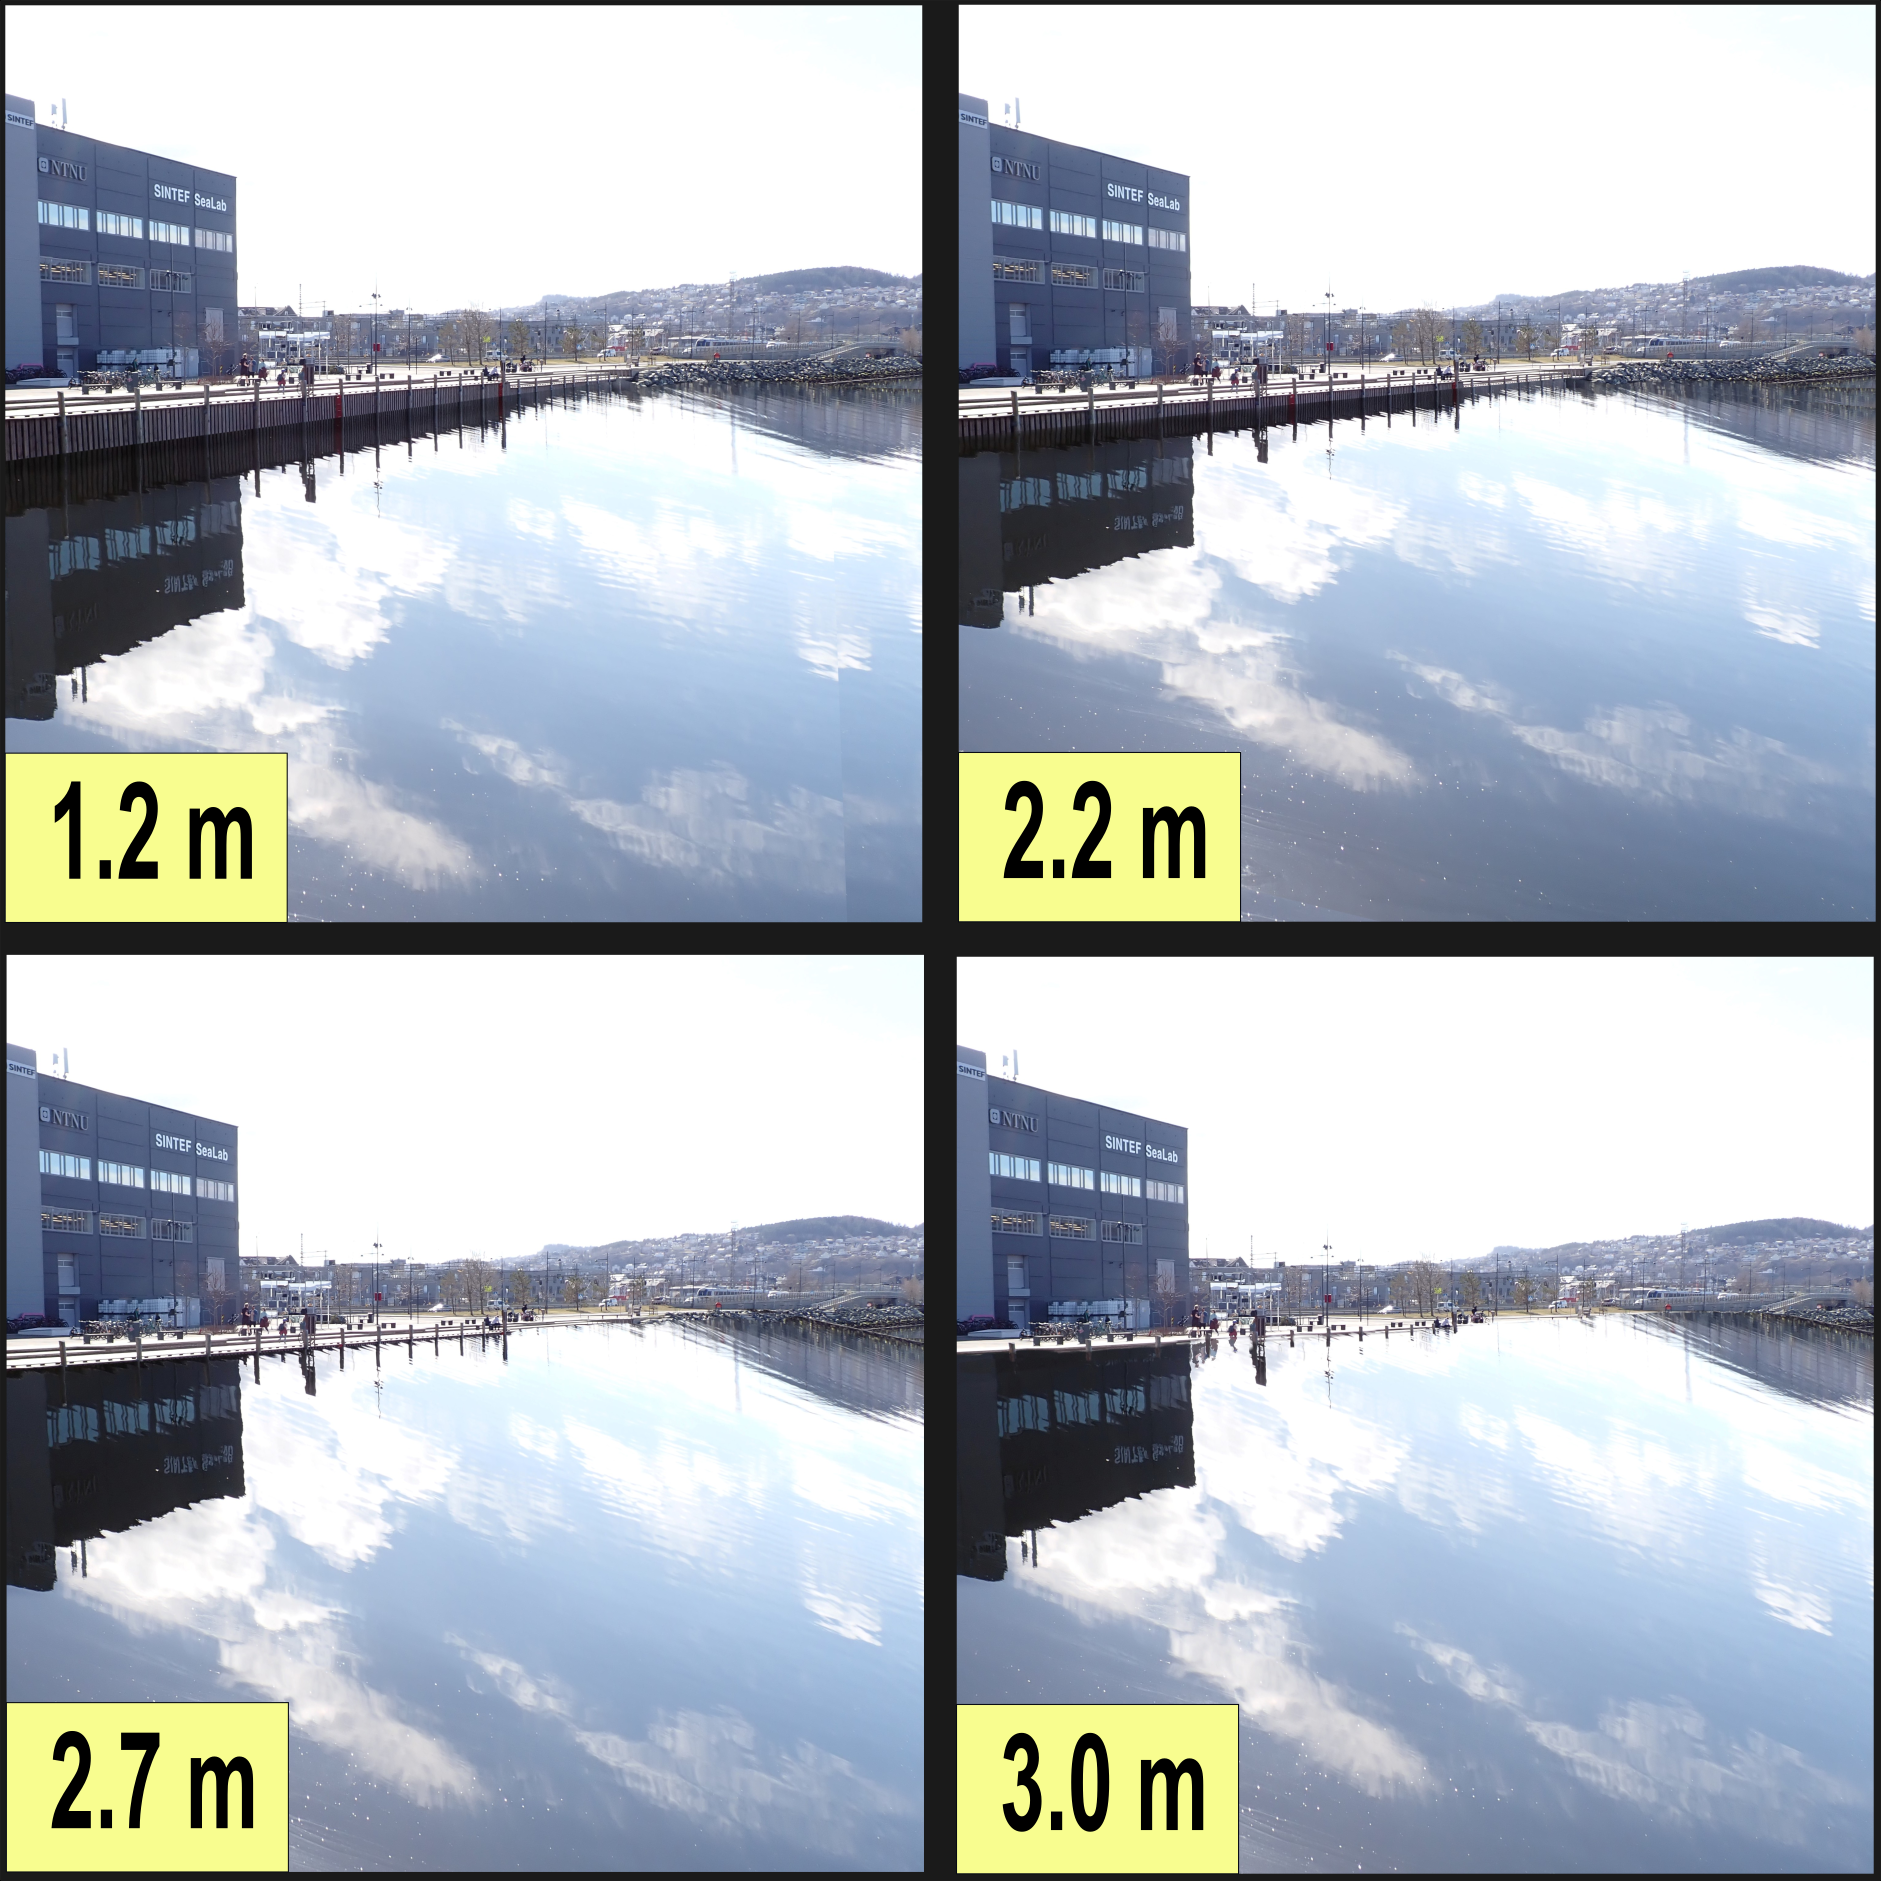
\includegraphics[width=1\textwidth]{fig_appendix/brattora 2090 q.png}
\paragraph{}
Hvilket bilde viser den nåværende 20-årene stormfloen?
\begin{itemize}
    \item 1.2 m
    \item 2.2 m
    \item 2.7 m
    \item 3.0 m
\end{itemize}
\paragraph{}

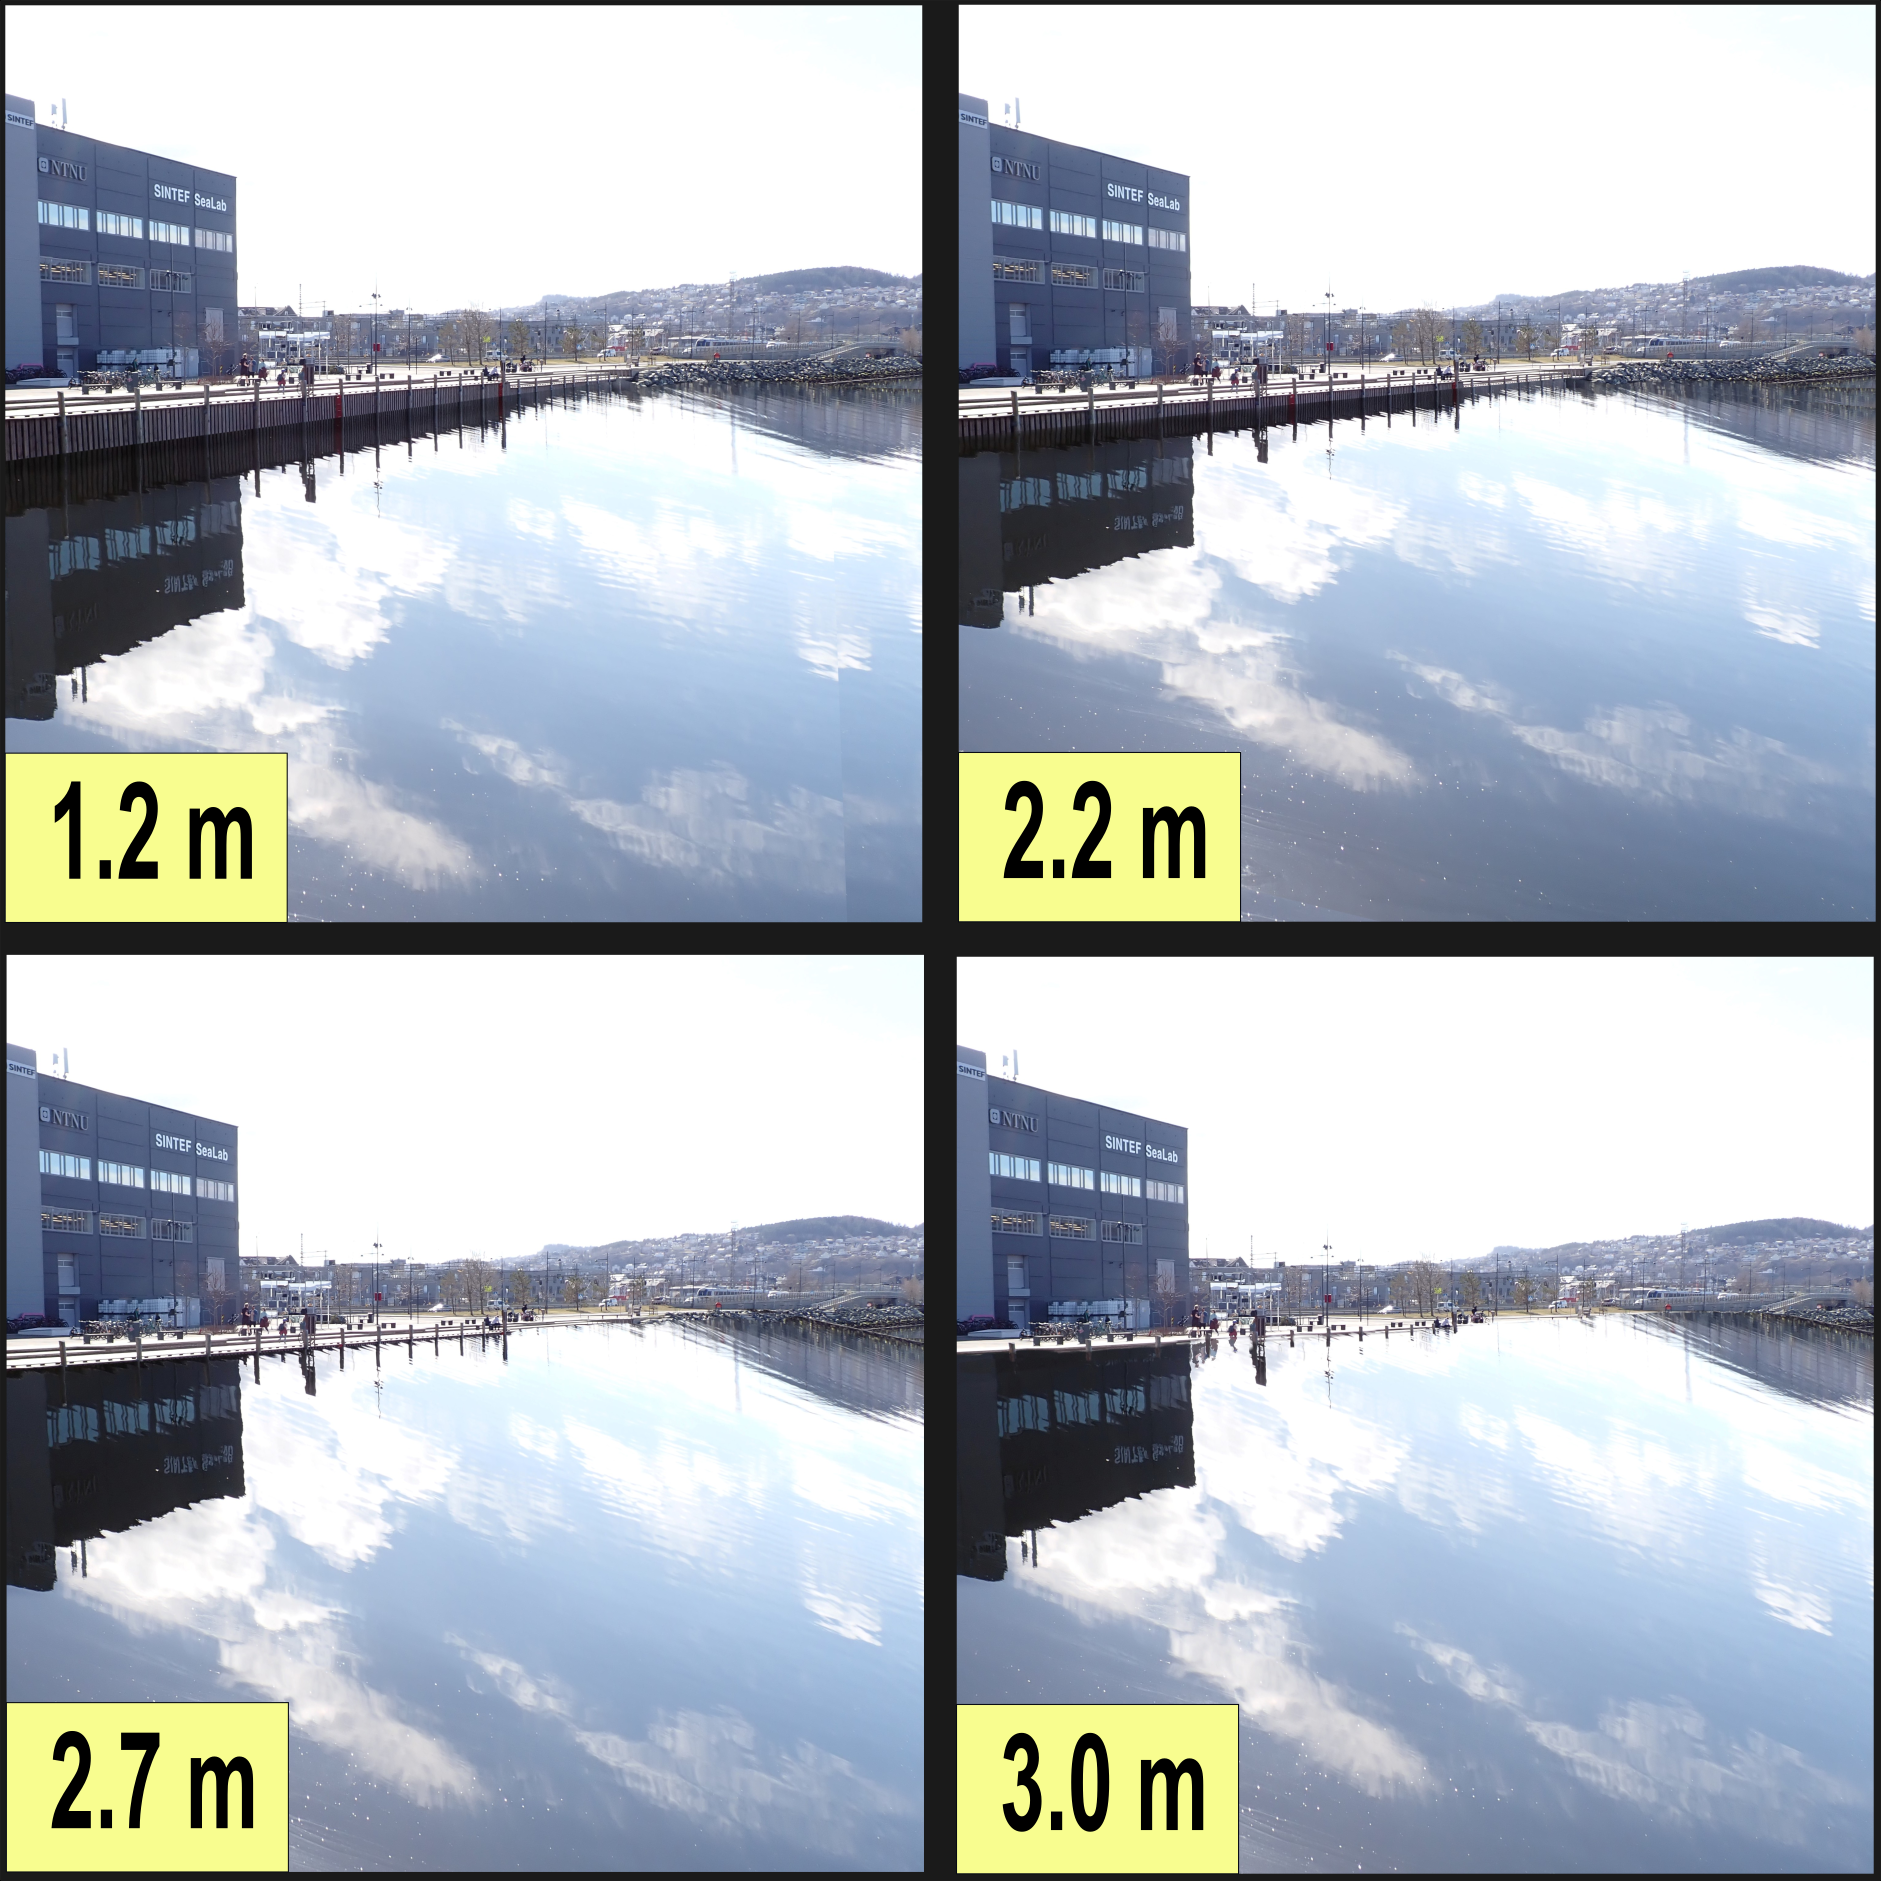
\includegraphics[width=1\textwidth]{fig_appendix/brattora 2090 q.png}
\paragraph{}
Hvilket bilde viser stedets 20-årene stormflo i 2090?
\begin{itemize}
    \item 1.2 m
    \item 2.2 m
    \item 2.7 m
    \item 3.0 m
\end{itemize}
\paragraph{}

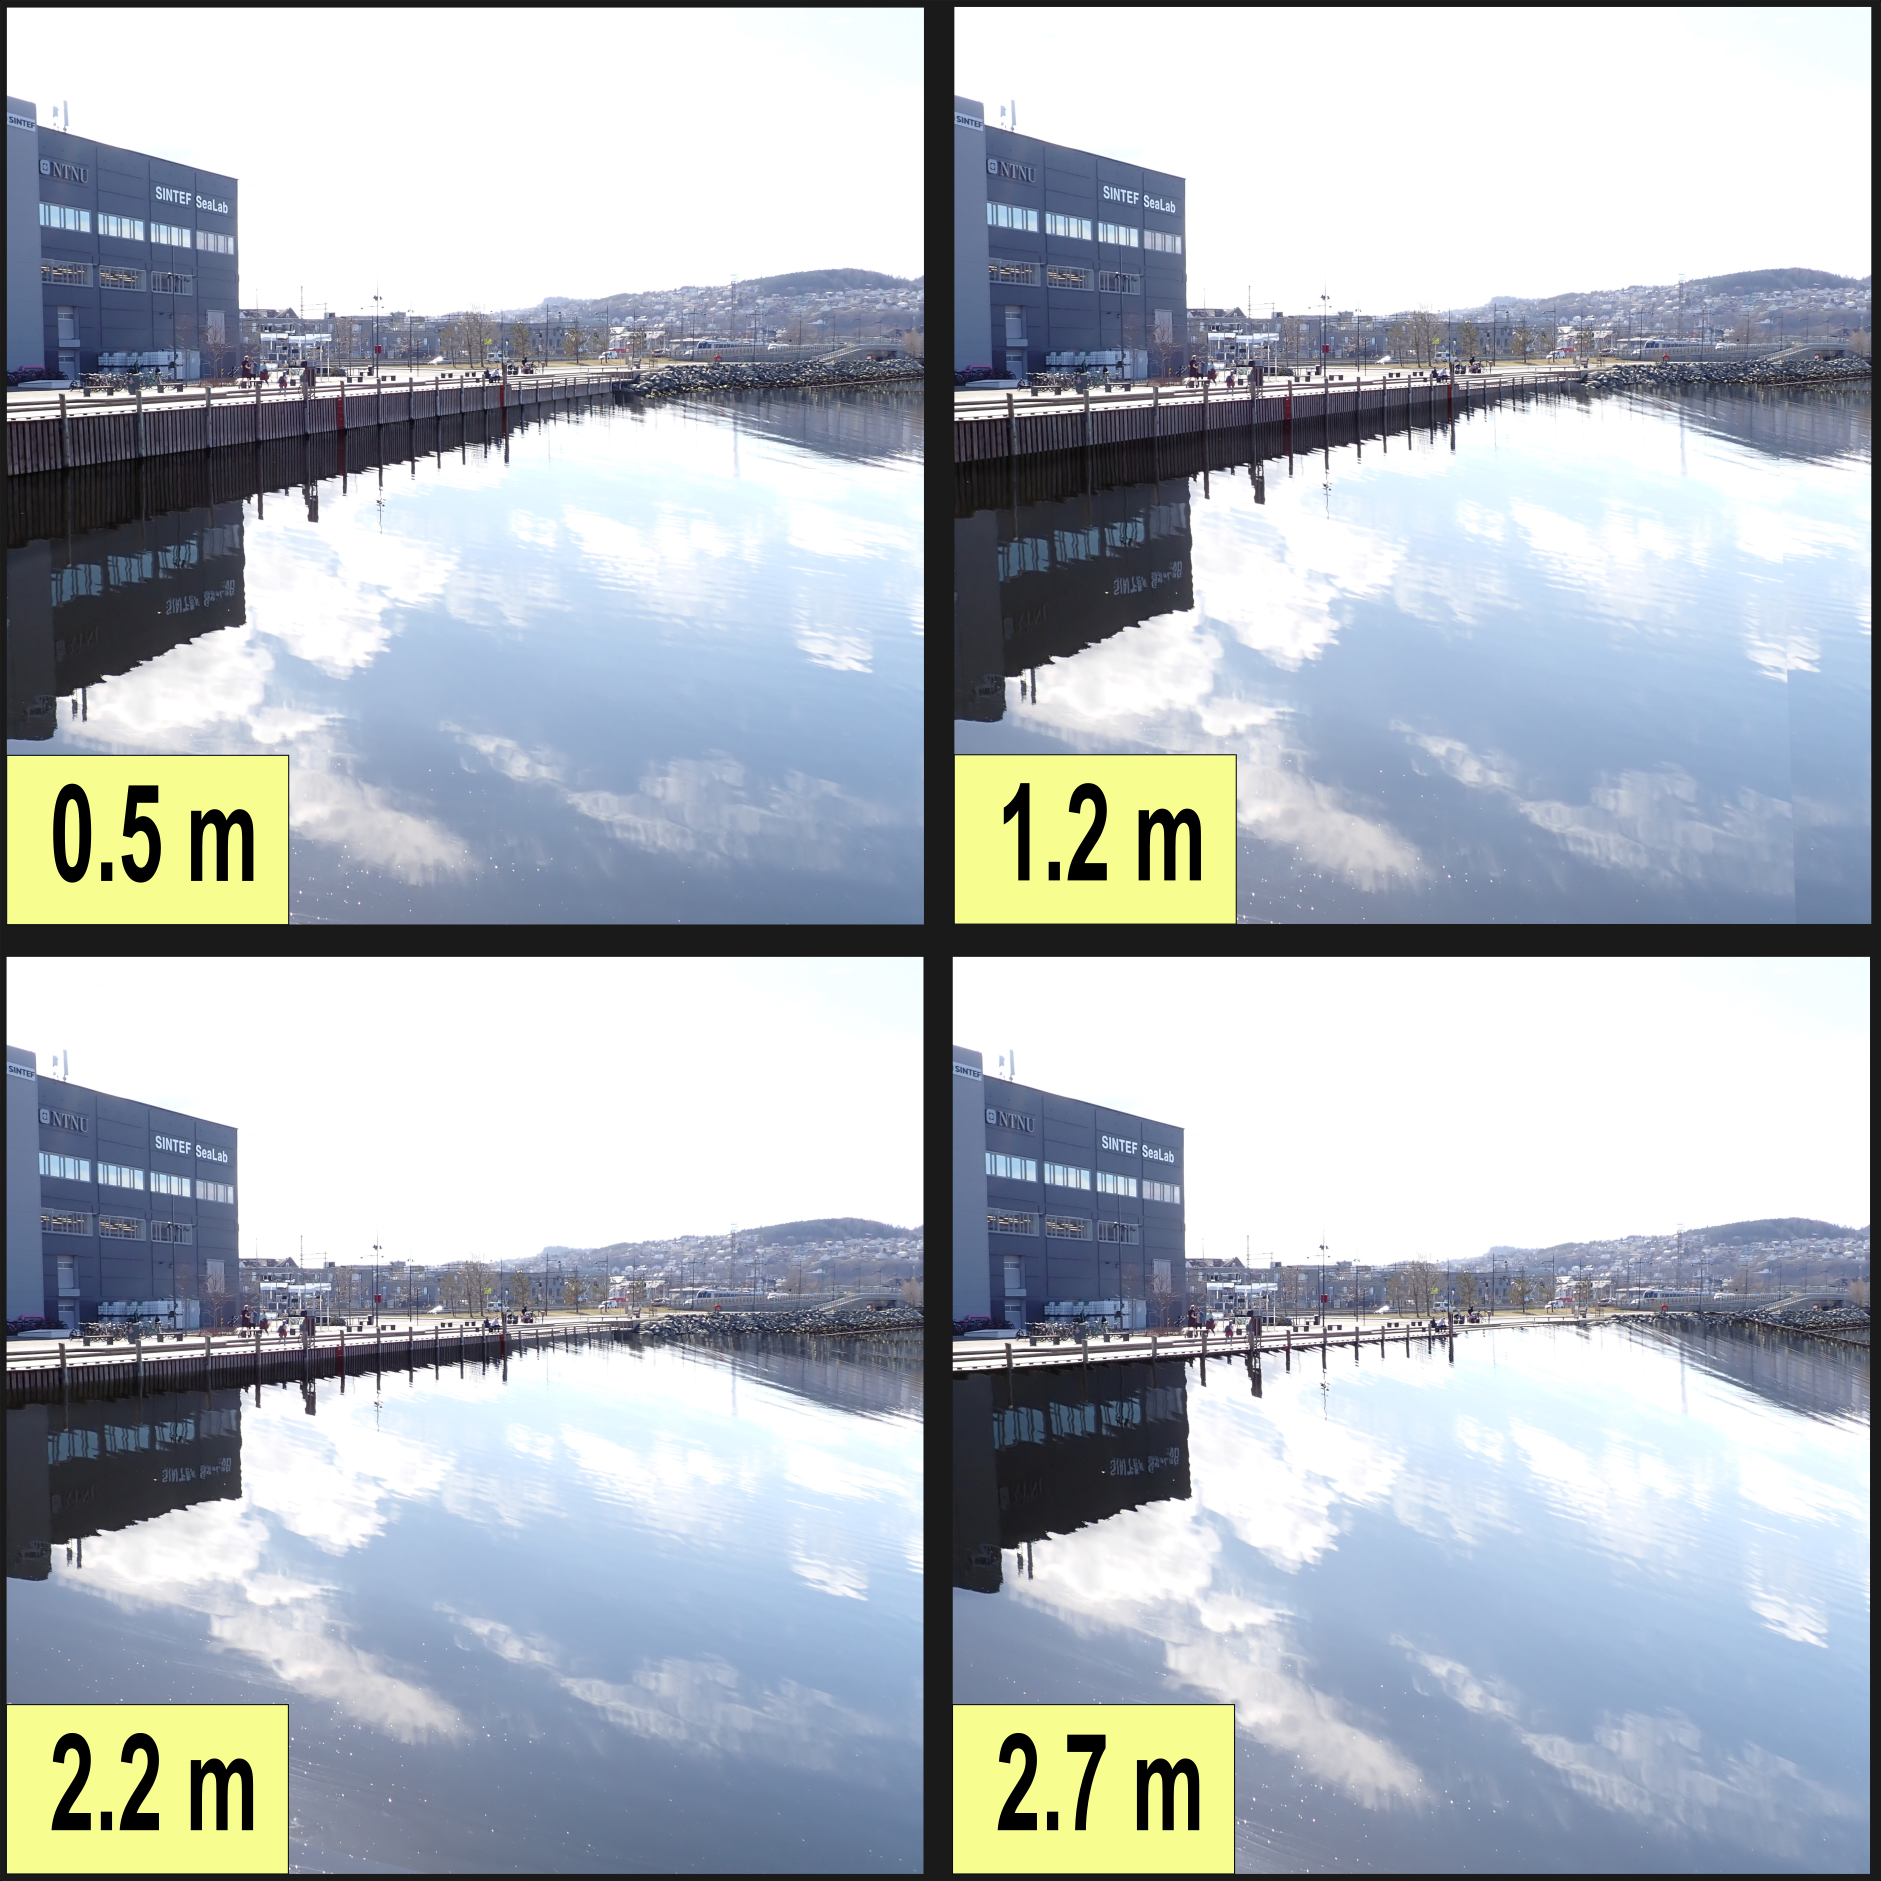
\includegraphics[width=1\textwidth]{fig_appendix/brattora 2022 q.png}
\paragraph{}
Hvilket bilde viser dette stedets høyvann i dag?
\begin{itemize}
    \item 0.5 m
    \item 1.2 m
    \item 2.2 m
    \item 2.7 m
\end{itemize}
\paragraph{}

Hvor får du informasjon om endringer på dette stedet?
f.eks. innsynkning, hendelser, veiarbeid
\begin{itemize}
    \item personlig observasjon
    \item familie
    \item venner
    \item aviser
    \item tv
    \item sosiale medier
    \item organisasjonsmedlem
\end{itemize}
\paragraph{}

Hvor får du informasjon om klimaendringer?
\begin{itemize}
    \item personlig observasjon
    \item familie
    \item venner
    \item aviser
    \item tv
    \item sosiale medier
    \item organisasjonsmedlem
    \item fagfellevurdert artikkel
    \item utdanning
\end{itemize}
\paragraph{}

Er du bekymret for klimaendringer?
1 - ikke i det hele tatt, 5 - veldig bekymret
Likertskala
\paragraph{}

Hvordan vil flom forbundet med ekstreme havnivåer i dette området påvirke deg?
\begin{itemize}
    \item ingen innvirkning
   \item mild innvirkning
   \item middels innvirkning
   \item høy innvirkning
\end{itemize}
\paragraph{}
Hvis du ønsker å gi flere detaljer om dette, vennligst skriv nedenfor
\paragraph{}

Hvor mye tror du havnivået har endret seg her de siste 30 årene?
(cm)
\begin{itemize}
    \item + 50 cm
    \item + 20 cm
    \item + 10 cm
    \item no change
    \item - 10 cm
    \item - 20 cm 
    \item - 50 cm 
\end{itemize}
\paragraph{}

Hvor mye tror du havnivået vil endre seg de neste 30 årene?
(cm)
\begin{itemize}
    \item + 50 cm
    \item + 20 cm
    \item + 10 cm
    \item no change
    \item - 10 cm
    \item - 20 cm 
    \item - 50 cm 
\end{itemize}
\paragraph{}

Kryss av hvis du husker disse ekstreme havnivå hendelsene.
Dette er alle datoene er havnivået i Trondheim har vært over 2 meter siden 1950.
\begin{itemize}
    \item 2020 februar
    \item 2011 november
    \item 1999 november
    \item 1998 februar
    \item 1997 februar
    \item 1993 januar
    \item 1990 februar
    \item 1971 november
\end{itemize}
\paragraph{}

Hva er de største risikoene for mennesker i dette området?
\begin{itemize}
    \item strandlinje ustabilitet
    \item stormflo
    \item bølger
    \item sterke vinder
    \item sterkt tidevann
    \item drukning
    \item kaldt vann sjokk
    \item Jeg vet ikke
    \item Jeg ser ingen store risikoer
    \item menneskelig feil
\end{itemize}
\paragraph{}

Hva er de største risikoene for infrastrukturen i dette området?
\begin{itemize}
    \item strandlinje ustabilitet
    \item stormflo
    \item bølger
    \item sterke vinder
    \item sterkt tidevann
    \item Jeg vet ikke
    \item Jeg ser ingen store risikoer
    \item forvitring
    \item nedbør
    \item menneskelig feil
\end{itemize}
\paragraph{}

Hvis du vil gi andre eksempler på risiko på dette området, vennligst skriv her.
\paragraph{}

Hvordan fikk du tilgang til denne undersøkelsen?
\begin{itemize}
    \item plakat
    \item e-post
    \item sosiale medier
    \item organisasjonsmedlem
    \item arbeidssted
    \item personlig tilknytning til forsker
\end{itemize}
\paragraph{}

Hvis du ønsker mer informasjon om denne forskningen, vennligst oppgi e-postadressen din.